\section{A Hand-on Guideline for Test-time Scaling}
\label{sec:handon}
In this section, we shift from theoretical categorizations to providing a practical, hands-on guideline for \textit{TTS}. Our goal is to offer clear, actionable instructions and technical pathways to facilitate effective SST deployment.

\begin{QABox}[Common Problems]

\Q{What kind of task does \TTS help?}

\A{Almost any task! While traditional reasoning tasks—such as Olympiad-level mathematics, complex coding, and game-based challenges—have been shown to significantly improve with \TTS, community observations suggest that \TTS can also enhance performance in open-ended tasks, such as comment generation or evaluation. However, due to the long-form nature of outputs and the lack of centralized, objective benchmarks, these tasks are inherently more difficult to evaluate quantitatively, making it harder to draw conclusive claims.
Beyond that, more realistic, complex, and long-horizon scenarios, like medical reasoning and law, have also shown promising gains through \TTS strategies.}

\vspace{1em}

\Q{If I want to quickly implement a \TTS pipeline, what are the essential paths I should consider? How can beginners use \TTS at a minimal cost?
}

\A{
Broadly speaking, there are three essential technical pathways for test-time scaling: i) Deliberate reasoning procedure at inference time, ii) imitating complex reasoning trajectories, and iii) RL-based incentivization. 
If your goal is to get a quick sense of the potential upper bound that a strong \TTS can bring to your task at a minimum cost, you can directly utilize a model that has been trained with (iii). If you want to develop a \TTS baseline at a minimum cost, you can start with (i). Once (i) yields a result that meets expectations, you can apply (ii) to further verify and generalize the outcome.
}

\vspace{1em}

\Q{Are these pipelines mutually exclusive? How should I design a frontier-level \TTS strategy?
}

\A{
These pipelines are by no means mutually exclusive—they can be seamlessly integrated. For instance, R1 inherently necessitates SFT through rejection sampling as a preliminary warmup step. When employing RL, practitioners should continue leveraging synthesized CoT methods and introduce additional structured inference strategies to tackle increasingly complex scenarios effectively. 
}
\vspace{1em}

\Q{What are some representative or widely-used \TTS methods that can serve as baselines?
}

\A{Parallel--Self-Consistency, Best-of-N; Sequential--STaR, Self-Refine, PRM; Hybrid--MCTS, ToT; Internal--Distilled-R1, R1.
}

\vspace{1em}

\Q{Is there an optimal go-to solution so far?
}

\A{No free lunch. Optimal computing is often dependent on the hardness and openness of the question.
}

\vspace{1em}

\Q{How should we evaluate the performance of a \TTS method? In addition to standard accuracy, what other aspects should we pay attention to?
}

\A{The evaluation is largely task-aware, but metrics like accuracy remain the most critical indicators. In addition, efficiency (the trade-off between performance and cost) is another key concern in practical settings. As \TTS becomes a more general-purpose strategy, researchers have also begun evaluating a range of secondary attributes, including robustness, safety, bias, and interpretability, to better understand the broader impacts of \TTS.
}

\vspace{1em}

\Q{Is there any difference when tuning other scaling formats into internal scaling, compared with directly using the original scaling format?
}

\A{Yes, one intuitive difference lies in the efficiency aspect. Internal scaling tends to yield higher efficiency as it only prompts the LM once, while other scaling techniques usually require multiple trials. However, internal scaling requires non-neglectable resources for tuning, making it less available for practitioners.}

\end{QABox}





% \begin{figure}[!htbp]
%   \centering
%   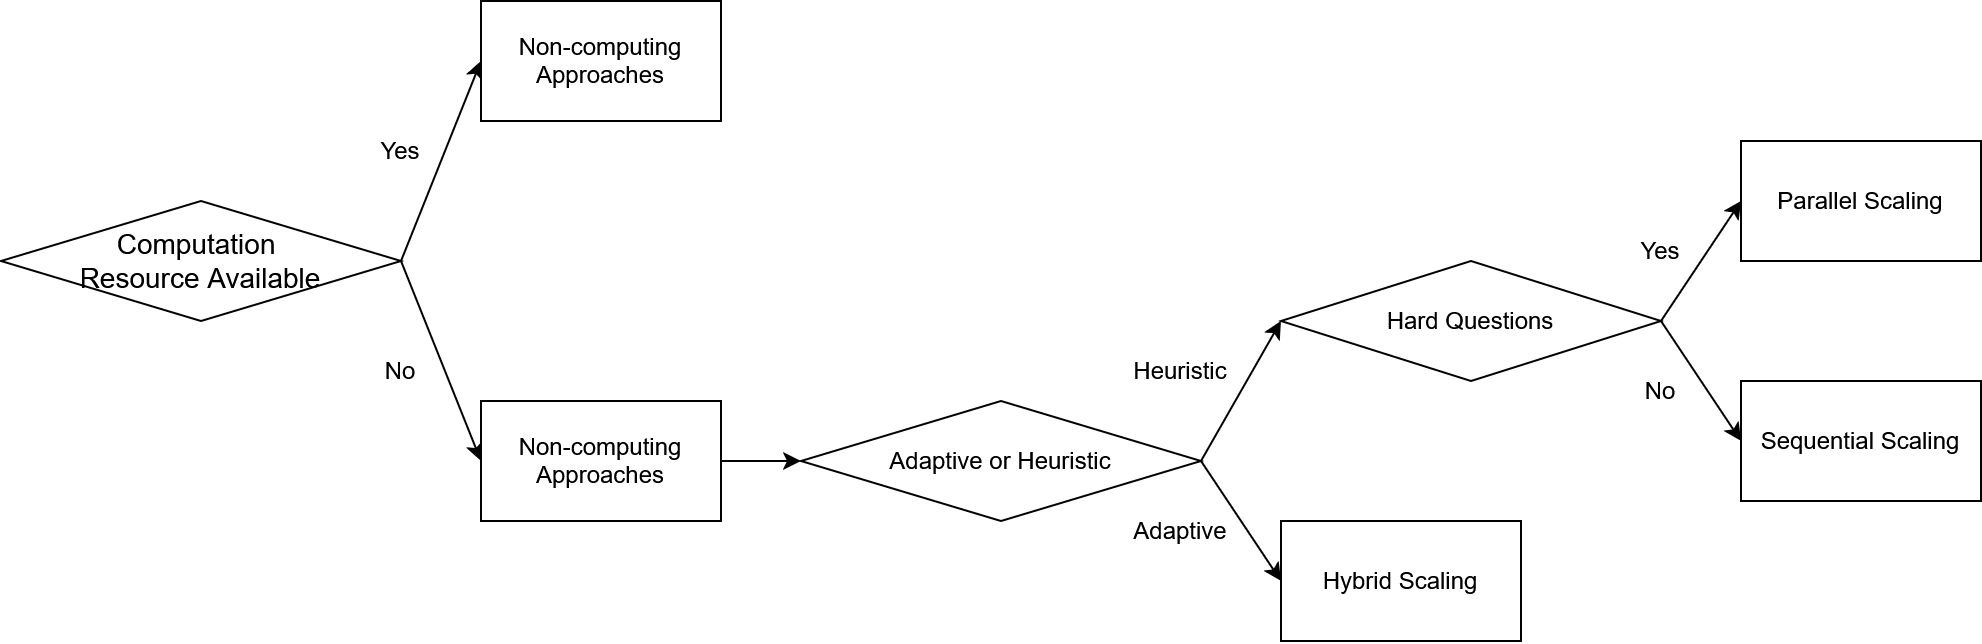
\includegraphics[width=0.98\textwidth]{figures/TTS-handon.png}
%   \caption{Hand-on Guideline for Test-time Scaling.}
%   \label{fig:tts-handon}
% \end{figure}


% =========== Fuyuan ===========

%Q2: Is there a way to test the effectiveness of test-time scaling with minimum effort?
%(How can beginners use \TTS at a minimal cost?)

%Q3: Is there an optimal go-to solution so far? (No, optimal computing is data-dependent)

%Q4: How stable is the \TTS solution compared to naive prompting?

% Q5: Is there any difference when tuning other scaling formats into internal scaling, compared with directly using the original scaling format? (This is also sth. I am interested)

% Q6: How does the connection
